%\documentclass[PhD,two side]{srmuthesis}
%\documentclass[MS]{srmuthesis}
%\documentclass[MTech]{srmuthesis}
\documentclass[BTech]{srmuthesis}
\usepackage{times}
\usepackage{t1enc}
\usepackage{tikz}
\usepackage{subfigure}
\usepackage{pgfplots}
\usepackage{setspace} 
\usepackage{geometry}
\usepackage{graphicx}
\usepackage{epstopdf}
\usepackage{lscape}
\usepackage{fancyhdr}
\usepackage{natbib}
\usepackage{hyperref} % hyperlinks for references.
\usepackage{amsmath} % easier math formulae, align, subequations \ldots
\usepackage{amssymb}
\usepackage{wasysym}
\usepackage{titlesec}
\usepackage{textcomp}
\usepackage{pifont}
\usepackage{appendix} 
\usepackage{float}
\usetikzlibrary{decorations.pathmorphing}
\usetikzlibrary{shapes,arrows,shadows,patterns}
\usepackage[printonlyused]{acronym}
%\usepackage{nomencl}
%\newcommand{\bigsize}{\fontsize{16pt}{20pt}\selectfont}
%\renewcommand\nomname{\centerline {NOTATION}}
%\makenomenclature
\setcounter{MaxMatrixCols}{20}
\captionsetup[figure]{labelfont=bf}
\begin{document}
%%%%%%%%%%%%%%%%%%%%%%%%%%%%%%%%%%%%%%%%%%%%%%%%%%%%%%%%%%%%%%%%%%%%%%
% Title page

\title{Intelligent Blood Bank Management System with integrated Decision Making System} % Enter The Project Title

\firstauthor{AYUSH SINGH}% Enter The Student name
\firstauthorregno{[Reg No: RA1511008010221]}
\secondauthor{ADITYA RAJPUT}% Enter The Student name
\secondauthorregno{[Reg No: RA1511008010237]}
\thirdauthor{REEZ PATEL} % If there is no third author, leave the space blank like \thirdauthor{}
\thirdauthorregno{[Reg No: RA1511008010255]}
\fourthauthor{MONISH DE}
\fourthauthorregno{[Reg No: RA1511008010261]}
\fifthauthor{SHREYA DHAGA}
\fifthauthorregno{[Reg No: RA1511008010295]}
\guide{Mr. K. Navin} % Enter your guide's name
\designation{Asst. Professor} % Enter your guide's designation
\guidedepartment{Information Technology} % Enter the department name of your Guide 
\hod{Dr. G. Vadivu} % Enter HOD's name
\department{Information Technology} % Enter your department name
\date{APRIL 2019} % Enter month and year of submission
%\nocite{*}

\maketitle
%%%%%%%%%%%%%%%%%%%%%%%%%%%%%%%%%%%%%%%%%%%%%%%%%%%%%%%%%%%%%%%%%%%%%%
%\vspace*{3in}
%\begin{center}
%{\Huge Dedicated to my Parents}
%\end{center}
%%%%%%%%%%%%%%%%%%%%%%%%%%%%%%%%%%%%%%%%%%%%%%%%%%%%%%%%%%%%%%%%%%%%%%
% Certificate
\certificate

%\vspace*{0.5in}



%%%%%%%%%%%%%%%%%%%%%%%%%%%%%%%%%%%%%%%%%%%%%%%%%%%%%%%%%%%%%%%%%%%%%%
% Abstract

\abstract
\begin{doublespacing}
{\large\noindent This project is requested by The Rotary Blood Bank and classifies as an m-health project. This project is aimed to help blood banks to manage their inventory systems using modern solutions. Our project has been developed keeping in view of the blood banks and the people that work for them, we aim to provide for excellent user experience. Intelligent data entry and retrieval classifies are the essentials for every modern inventory system. The digital system design provides a context-dependent user interface that makes it easier for the transition. Using our system the blood stored within the blood banks can easily be tracked audited and used. To fetch and maintain audits is a big task in the blood banks, our system addresses this concern with a smart search solution. Managing data is easier and efficient and organized. This system provides you with basic analytics on the basis of your data. Duplication of data and the rising concern of illicit blood transfer in the red market is also addressed. There is the security of data and rights that are only given to the administrator, this system has access to specifiers and a distributed database system that makes it easier to expand for the future. We hope that this project can grow to become a standard for blood bank inventory systems across various regions. }
\end{doublespacing}

\pagebreak
%%%%%%%%%%%%%%%%%%%%%%%%%%%%%%%%%%%%%%%%%%%%%%%%%%%%%%%%%%%%%%%%%%%%%%
% Acknowledgements
\acknowledgements
I would like to express my deepest gratitude to, Mr Rajagopal Aravindan and the Rotary Blood bank for providing us with an opportunity to work in this healthcare project, and to my guide, Mr K. Navin for his valuable guidance, consistent encouragement, personal caring, timely help and providing me with an excellent atmosphere to accomplish this project. All through the work, in spite of his busy schedule, he has extended cheerful and cordial support to me for completing this work.

\begin{flushright}
{\bf Author}
\end{flushright}
%%%%%%%%%%%%%%%%%%%%%%%%%%%%%%%%%%%%%%%%%%%%%%%%%%%%%%%%%%%%%%%%%
% Table of contents etc.

\begin{singlespace}
\tableofcontents
\thispagestyle{empty}

\listoftables
\addcontentsline{toc}{chapter}{LIST OF TABLES}
\listoffigures
\addcontentsline{toc}{chapter}{LIST OF FIGURES}
\end{singlespace}


%%%%%%%%%%%%%%%%%%%%%%%%%%%%%%%%%%%%%%%%%%%%%%%%%%%%%%%%%%%%%%%%%%%%%%
\abbreviations
%\begin{acronym}[longest acronym must be entered here]
\begin{acronym}[OKID/ERA]

%\acro{acronym}{in detail}
\acro{ABC}{Artificial Bee Colony}
\acro{ACO}{Ant Colony Optimization}
\acro{BA}{Bees Algorithm}
\acro{BFO}{Bacterial Foraging Optimization}
\acro{BM} {Bending Moment}
\acro{CMIR}{Condensed Model Identification and Recovery}
\acro{CMTM}{Consistent Mass Transfer Matrix}
\acro{CPU}{Central Processing Unit}
\acro{CS}{Cuckoo Search}
\acro{CSI}{Complete Structural Identification}
\acro{DAQ}{Data Acquisition}
\acro{DOF}{Degrees Of Freedom}
\acro{DTM}{Damped Transfer Matrix}
\acro{EA}{Evolutionary Algorithm}
\acro{EKF}{Extended Kalman Filter}
\acro{ERA}{Eigen system Realization Algorithm}
\acro{FE}{Finite Element}
\acro{FRF}{Frequency Response Function}
\acro{GA}{Genetic Algorithm}
\acro{LCTM}{Lumped Crack Transfer Matrix}
\acro{LM}{Levenberg-Marquardt}
\acro{LMTM}{Lumped Mass Transfer Matrix}
\acro{LS}{Least Square}
\acro{MAE}{Mean Absolute Error}
\acro{MSE}{Mean Square Error}
\acro{MSI}{Modular Smart Interface}
\acro{OKID/ERA}{Observer Kalman Filter Identification/Eigen Realization Algorithm}
\acro{PSO}{ Particle Swarm Optimization}
\acro{SA}{Simulated Annealing}
\acro{SCTM}{Single Crack Transfer Matrix}
\acro{SF} {Shear Force}
\acro{SHM}{Structural Health Monitoring}
\acro{SI}{Structural Identification}
\acro{SS}{Sub-Structure}
\acro{SSI}{Sub-Structural Identification}
\acro{TCTM}{Two Crack Transfer Matrix}
\acro{TM}{Transfer Matrix}
\acro{HIV}{Human immunodeficiency virus}
\acro{HEP B}{hepatitis B}
\acro{HEP C}{hepatitis C}
\acro{MP}{Mucopolysaccharidosis}
\acro{VDRL}{Venereal Disease Research Laboratory}
\acro{ACID}{Atomicity, Consistency, Isolation, Durability}
\acro{SQL}{Structured Query Language}
\acro{NN}{Neural Network}
\acro{MERN}{MongoDB, Express, React, Node}
\acro{PUS}{Purchased, Used and Stock}
\acro{KPI}{Key Perfromance Indicators}
\acro{DOB}{Date of birth}
\acro{JSON}{JavaScript Object Notation}
\acro{API}{Application Program Interface}
\acro{REST}{Representational State Transfer}
\acro{HTTP}{Hyper Text Transfer Protocol}
\end{acronym}
% Use the syntax \ac{acronym} whereever you use this acronym.
% Abbreviations

%\noindent 
%\begin{tabbing}
%xxxxxxxxxxx \= xxxxxxxxxxxxxxxxxxxxxxxxxxxxxxxxxxxxxxxxxxxxxxxx \kill
%\textbf{TM}   \> Transfer Matrix \\
%\textbf{LMTM} \> Lumped Mass Transfer matrix \\
%\textbf{CMTM} \> Consistent Mass Transfer matrix \\
%\textbf{SCTM} \> Single Crack Transfer matrix \\
%\textbf{LCTM} \> Lumped Crack Transfer matrix \\
%\textbf{DCTM} \> Double Crack Transfer matrix \\
%\textbf{DOF} \> Degrees Of Freedom \\
%\textbf{GA} \> Genetic Algorithm  \\
%\textbf{PSO} \> Particle Swarm Optimization \\
%\textbf{SI} \> Structural Identification \\
%\end{tabbing}

\pagebreak

%%%%%%%%%%%%%%%%%%%%%%%%%%%%%%%%%%%%%%%%%%%%%%%%%%%%%%%%%%%%%%%%%%%%%%
% Enter the symbols used in the thesis in alphabatical order
\chapter*{\centerline{LIST OF SYMBOLS}}
\addcontentsline{toc}{chapter}{LIST OF SYMBOLS}

\begin{doublespace}
\begin{tabbing}
%\printnomenclature
xxxxxxxxxxx \= xxxxxxxxxxxxxxxxxxxxxxxxxxxxxxxxxxxxxxxxxxxxxxxx \kill
\textbf{$\omega$} \> Probability \\
\textbf{$\sigma$} \> Standard Deviation \\
\textbf{$\mu$} \> Mean \\
\textbf{$\sum$} \> Summation \\

\end{tabbing}
\end{doublespace}

\pagebreak
\clearpage
% The main text will follow from this point so set the page numbering
% to arabic from here on.
\pagenumbering{arabic}


%%%%%%%%%%%%%%%%%%%%%%%%%%%%%%%%%%%%%%%%%%%%%%%%%%
% Introduction.

%Enter your chapter number here
\chapter{INTRODUCTION}
\label{chap:intro}
Blood donation is a voluntary procedure. A person can give their blood to someone who may need a transfusion. Millions of people need blood transfusions each year. Some may need blood during surgery. When we go to give blood we will be asked to perform simple tests that will check our health state. When there is any problem in our health the test will discover it early and you can then have suitable health care and reassurance. After this state, the donation authorities take in the donor details and screen the blood. In the screening process, the donor’s blood type is identified and it is checked for infections like \ac{HIV}, \ac{HEP B}, \ac{HEP C}, \ac{MP}, and \ac{VDRL}. The blood is usually discarded of any of these tests are positive. After the initial screening, the blood is taken from the candidate and stored in the banks in optimal conditions. This whole system including the storage and feeding the data is done through registers manually.\par 
This is a time taking process and often leads to many errors due to wrong blood transfusions or incorrect samples being sent to the hospitals from the blood banks. This also leads to accounting mismanagement and illegal trafficking of blood in the red market reports according to BBC. 
\section{Insight to Database Management Systems}
In the current world, we have a lot of raw data that can be processed and kept in a systematic manner to retrieve information. A Database is this type of collection of information. Databases help in making the project easily accessible, manageable and update-able. Data is organized into tables, each table has rows and columns. Data is indexed to find relevant information. Database processes help to create and update them through the use of queries. A query is an action of retrieving data from a database. Computer databases contain data of large records or filed that can indefinitely expand provided the hardware is available.\par 
Typically, a database manager provides the user with the ability to control some part of the data, these are known as access levels or user permissions. User Permits are put in place to keep data secure and abstract a portion of the database. A good database offers \ac{ACID} compliance to guarantee that data is consistent. The Database Management Systems serves an interface between the database and end users or application programmers, to ensure that data is easily accessible. A database is useful for providing a central view of data that is organized and quantified, as well as ensuring there is no redundancy in the database. 
\section{Types of Database Management Systems}
Databases Management Systems can be done using various languages and procedures. Following give the basic types of classifications.
\subsection{On the basis of the data model} 
\subsubsection{a. Relational Database}
A relational database is a database that has a collective set of many datasets organized using tables, records and columns. These databases ensure that there is a well-defined relation between different databases tables. These tables share information which facilitates search, organization and reporting.
These Databases are backed by usage of \ac{SQL}, which is usually a standard.
\begin{figure}[h!]
	\centering
	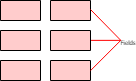
\includegraphics[scale=1.0]{Fields.png}
	\caption{Fields}
\end{figure}
\begin{figure}[h!]
	\centering
	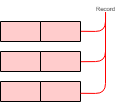
\includegraphics[scale=1.0]{Record.png}
	\caption{Record}
\end{figure}
\begin{figure}[h!]
	\centering
	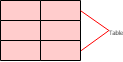
\includegraphics[scale=1.0]{Table.png}
	\caption{Table}
\end{figure}
\subsubsection{b. Object Oriented Database}
An object-oriented database is a database that allows the definition of objects, which is different from normal database objects. These systems subscribe to the model with the information shown by objects. Objects refer to the ability to develop a product and then define and name it, this enables the object to be referenced as a unit without having complex system involvement.
\begin{figure}[h!]
	\centering
	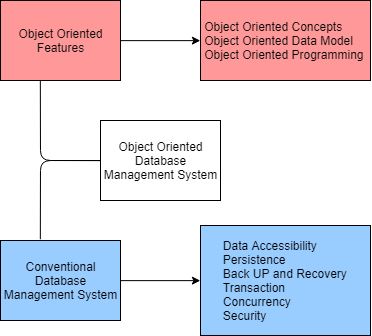
\includegraphics[scale=0.7]{OODB.png}
	\caption{Object Oriented Database}
\end{figure}
\subsubsection{c. Object Relational Database}
An Object Relational Database is a database management system that has components of both relational and object-oriented components. Object Relational Databases support the basic components of an object-oriented database model in schema and queries. It takes characteristics from both the Relational and Object Oriented Models.
\begin{figure}[h!]
	\centering
	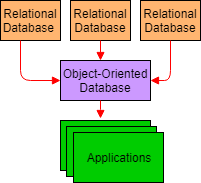
\includegraphics[scale=1.0]{ORD.png}
	\caption{Object Relational Database}
\end{figure}
\subsubsection{d. Hierarchical Database}
A hierarchical database is a database that shows a one-to-many relationship of a database and therefore is in a tree-like representation. These links elements to a parent/primary record.
\begin{figure}[h!]
	\centering
	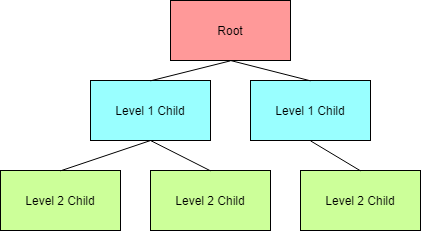
\includegraphics[scale=0.7]{HierarchialDB.png}
	\caption{Hierarchial Database}
\end{figure}
\subsubsection{e. Network Database}
A Network Database is a database that shows many-to-many relations and therefore allows multiple parent multiple child records in the database. Essentially it forms a net-like structure.
\begin{figure}[h!]
	\centering
	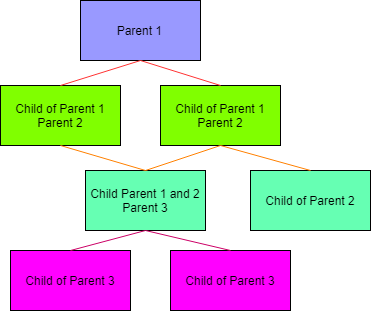
\includegraphics[scale=0.7]{NetworkDB.png}
	\caption{Network Database}
\end{figure}
\subsection{On basis of users}
\subsubsection{a. Single User Database}
A Single User Database allows only one connection to the database at a given point of time. This means that only one user is allowed to connect to the database throughout the server at a given moment of time.
\subsubsection{b. Multiple Users Database}
A Multiple User Database allows more than one connection to the database at a given point if time.
\subsection{On the basis of sites over which network is distributed}
\subsubsection{a. Centralized Database System}
A centralized database system has a single processor with its storage devices and other peripherals, due to this it is physically confined to a location. Data can be accessed from many sites using a single network while the maintenance is on a single site. 
\begin{figure}[h!]
	\centering
	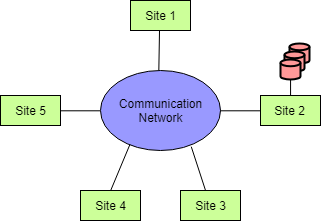
\includegraphics[scale=0.7]{CenterslizedDB.png}
	\caption{Centralized Database System}
\end{figure}
\subsubsection{b. Parallel Network Database System}
A parallel database system has multiple processing units and disks storage is in parallel. This improves the input/output speed and therefore are used in the application that has to query large transaction rates.
\subsubsection{c. Distributed Database System}
A distributed database system is a system that is spread over different sites. These locations don’t share physical components and are accessed globally by all users. Although it should be noted that for the user it must look as if it were one single database. It is classified as Homogeneous Database and Heterogeneous Database.
\begin{figure}[h!]
	\centering
	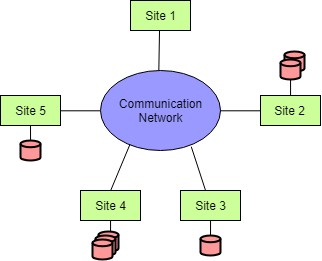
\includegraphics[scale=0.7]{DistributedDBMS.png}
	\caption{Distributed Database System}
\end{figure}
\section{Blood Bank Inventory Management}
In this project, we are using a centralized database system that helps keep a single database. The data first goes from the blood banks to the front end application developed through react framework. After basic validation tests, it goes through cloud-based support on Amazon Web Services and finally it is passed to the database.
\begin{figure}[h!]
	\centering
	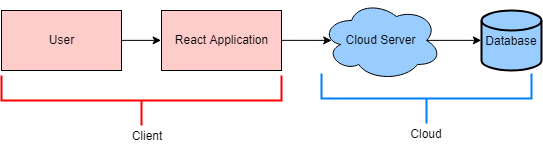
\includegraphics[scale=0.7]{BBInventoryManagement.png}
	\caption{Blood Bank Inventory Management}
\end{figure}
\section{Importance of shift}
There has been a trend in the increase in the gap of the demand-supply ratio of blood and organ donation. According to the articles and reports, this change in the trend is attributed to the high accounting management in the blood banks and selling of quints of blood in the red market. To fraud a few quints of donated blood and then changing the given blood by taking more blood from the same donor but not registering them, such people manage to sell blood.\par 
There is no security of users personal data. Audits are often slow tedious and have errors. In a survey, it shows that there is an 0.2\% error rate of wrong blood. While 0.2 may not seem a large number out of every 100 people, 2 people die just because they could not receive the blood they needed. These are present because of the manual system and can be eliminated with the use of a digital system.
\section{Accomplishment}
This project encourages the use of Human-Computer-Interface. The user interface and the user experience with the system have seen a positive response. Along with increased precision, less storage space and ease of audits, we have created a simple and easy to use interface keeping the users in minds.


\chapter{LITERATURE SURVEY}
\label{chap:literature}
\section{Blood for sale: India’s illegal ‘red market’}
According to the World Health Organization, which states the standards for blood reserves to be 1\% for every country states that there is a chronic short supply in India. India needs 12 million blood units annually instead ends up a collection of only 9 million units only. This accounts for a 25\% deficit. A trend shows that this deficit percent rises to 50\% leading to a spur of desperate patients. The lack of a central accounting along with a reluctance to donate blood accounts for the shortage. In 1996 Supreme Court running banned unlicensed blood banks but a little has changed from those times. Demands still outstrip supply. The illicit market has simply moved underground. A large sum of Blood is supplied to these markets because records are accessible to manipulate and change to everyone and not secure. A digital inventory will ensure that this accounting mismanagement does not happen. \cite{bbcarticle}
\section{Database Lifecycle}
The database life cycle comprises of six phases, each of which is essential to the making of a stable database and organize information curated to individual needs. Phase 1 is the Initial study which is to analyze, define the problem and list the objective scope and boundaries of the problem. Phase 2 is the Database Design phase, this is loosely related to designing the larger architecture, this is to figure out where the data will fit in the grander scheme of the project. Phase 3 is the Implementation and Loading of the database this phase includes the creation of tables, attributes, views, domains, indexes and many other constraints including security and performance guidelines. Phase 4 is the Testing and Evaluation here the project is run and tested, all current errors and cases are handled. Phase 5 is Maintenance and Evolution this includes developing means for backup and recovery, Active maintenance of new and old users. \cite{data_managemenet_life_cycle}
\section{Concepts of Database Management Systems}
Database Management System is a platform for a lot of functions and services that it has to perform, which guarantee the integrity and consistency of the data that is provided. This inventory ensures that we provide management for permanent storage. The inside schema decides the process of storage management in the physical hardware of the system. The full task list of any database management system includes the basic ability to retrieve, update, delete and store data into respective databases. Our system also accepts external, internal and conceptual schemas with all associated mappings like all other database management systems. Every database management system must provide catalogue management to the user. The end users request for database access are transmitted, we ensure that there is no unauthorized access in this process. A part of our inventory management is focused on backup and recovery as it is an essential feature for every database management system. All database management systems provide an interface for applications to interact with them, we have used NoSQL. Using queries that have Data definition and data manipulation parts to use and access the database we have ensured that the current system has all the functionalities of a standard database management system. \cite{concept_of_database_mngmt}
\section{The Ultimate Guide to SDLC}
Software Development Lifecycle is a series of definitive set of tasks performed to make software. It is followed by every development team that is making a software solution. There are several models that follow but with five essential steps. These are Planning, Defining, Designing, Testing, and Deploying. Many times a seven-step model is seen that includes recovery and maintenance in addition to the above five-step process. A variation of these steps is seen in models like the Waterfall model, V model, Incremental model, Iterative model, Spiral model, and the Big bang modal. \cite{sdlc_book}
\section{ReactJS}
React is a complete javascript library that is used to make user interfaces. It is used to make the frontend of our application. Developed by Facebook, react is a component-based system and thus has more modules and concepts of objects.  This factor makes react easier to debug and makes the code more predictable. \cite{reactjs} \cite{nodejs}
\section{What Happens to Donated Blood}
This is an article that shows the insight upon how blood donation systems work and the requirements of an inventory. There are a total of six steps contributing to blood being successfully donated and used. First, you arrive at the donation center and your physical and medical checkup is cleared then health history is also noted your donated sample is made to undergo preliminary screening. Then in the second step blood is taken to the processing center where whole blood donations are spun in centrifuges. Due to spinning, we get three components that are Red cells, Platelets and Plasma. Each component is packaged as a “unit”. Alongside the second step, the third step will take place a dozen tests will be performed on your blood and even if one of them turns out to be positive your blood is discarded. The test results arrive in the fourth step and the units are stored according to the prescribed conditions. Step five is the distribution of blood where it is necessary. Finally, the blood is transfused in the patient. \cite{redcross}
\section{MongoDB}
Mongo DB allows an easy organization, use and enrichment of data anywhere. It provides complete flexibility to the developer and seamless data migration. Mongo DB is a document database with a lot of scalability. 
The data is retrieved, manipulated and entered through the use of queries. Since the model maps application in application code it makes out retrieval and searching quick and efficient. It is a distributed database at its core so it is easier for horizontal searching. Moreover, Mongo DB is free to use. \cite{mongodb}
\section{Foundations of Software Testing}
Software Testing checks whether the actual results match the expected outcomes thereby ensuring that the application is defect free. It can also be called as Verification of Application Under Test. there are three broad classifications of testing mainly Functional testing, Non-functional testing, and Maintenance testing. There are seven principles to software testing which are keenly observed and implemented during the course. Software Testing Life Cycle goes hand in hand in with the development lifecycle and therefore is a part of the waterfall and the v model. This includes the Requirement analysis, Test Planning, Test case Development, Environment Setup, Test Execution, and Test Cycle Closure. Each of these stages has entry criteria and exit criteria. Testing can be done manually and automatically depending upon the application and the test cases it covers. Apache Jmeter is used for automatic testing. It is a pure Java open source. It is mainly used on performance testing and to analyze all tests. Jmeter simulates a bunch of user requests to the server that is targeted and returns information by analyzing these results.
\section{Box Detection Algorithm}
This algorithm enables us to detect any table format and extract the data from it using simple morphological operations. To do this for any image we first use preprocessing, in this project preprocessing means to extract the location of where our box is located. Then we can subject this image through the algorithm. To extract each cell one by one and detect the numbers we will apply the Machine Learning model to do the recognition. First, we convert the image to grayscale and then we perform thresholding and inversion. We then have two kernels operate on the same image. One is used to detect the horizontal lines the other is used to detect vertical lines. These two complete our basic morphological detection and the end result is that we have two images. We then add these two images to recreate the box, this removes all the noise present in the image preventing false box detection. After finding all boxes we will sort these using containers then crop them and put them in a folder or subject them to further processes. \cite{boxdetectionalgo}
\section{Offline Handwriting Recognition Using a Generic Algorithm}
The handwritten document is scanned as input to obtain individual characters. These are written in a text file and are later read back. After this, they are passed back to \ac{NN}. The scanned grayscale image is read into a matrix which is converted to a monochromatic image matrix with pixel values of 0 for black and 255 for white points. A process of row-wise searching is done from the point (0, 0) to find out the first black point. This is the upper point. After this point, all points are connected to this black value of 999. Post this the values having 999 are connected to recreate the word. The lowest point is now found out and the rightmost and leftmost points are obtained. Then we determined that no letters are missing. Word is searched for the number of cuts on a row-wise and column-wise manner. These are stitched again to recreate the word. \cite{handwritingalgobook}


\chapter{System Analysis}
\section{Problem Definition}
Blood Bank Inventory management systems are challenging but necessary changes that need to be shifted to the digital platform. There is a need for setting a standard procedure to acquire and store blood in every blood bank. There is no effective digital blood banks management system that is currently being used in the blood banks. Whereas it is necessary to make this system sustainable and reliable. \cite{medium_design_process}
\section{Proposed System}
Through this project, we focus on helping blood bank employees and make their tasks easy while giving them analytics about their blood bank, patients as well as the clients which are the hospitals, thereby helping the process become faster and secure. We use a massive amount of real data to design our system. This is provided by the rotary blood bank including the test cases that come along with the system.\par 
The donor's data is analyzed carefully and upon different parameters, predictions are given to various centers. We have used all modern technologies in order to make sure easy maintenance and usage. We have made the system with a simple design keeping in mind that the end user may not be well versed in computers.\par 
This system plans to shift the current system to a digital platform from the manual records that are maintained. Intelligent data entry and retrieval supported by decision-making system for an integrated blood bank management is a web-based application that is scalable and sustainable to the current and future needs.
\subsection{Advantages of Proposed System}
The employees at the blood bank through this system will be able to perform their operational requirements more easily and efficiently thereby increasing their overall productivity. At the same time it will also bring a huge impact to the society and the patients who actually need blood, because it's about saving a life through technology which is an enormous break through towards humanity.\par 
Considering the real time requirements, enormous data and complexities of the system, we used a client server architecture where the systems deployed at the blood bank will be directly communication with a centralized server which will can be deployed on Amazon Web Services. On this server our Mongo Server will also be up and running all the time to fulfill the client's need.
\section{Requirements}
\subsection{Hardware Requirements}
CPU - Dual Core Intel Core i3 or Higher.
\newline
Ram - 2GB or Higher.
\newline
HDD - 30GB or Higher
\newline
Input Devices - Keyboard, Mouse.
\newline
Monitor - 15” (1366*768) or Higher
\subsection{Software Requirements}
\subsubsection{a. Server}
Ubuntu/Linux
\newline
MongoDB
\newline
Node
\newline
Express
\newline
React
\newline
TypeScript 
\newline
VS Code
\subsubsection{b. Client}
Windows 8 or Later
\section{Issues in existing methodology}
In the current system, records are maintained in registers, these registers are organized by the years, monthly donor data in huge racks and other records. This system is not only redundant and slow but also consumes a lot of space and makes it tough to maintain huge amounts of data. The current system cannot sustain the urgency of blood donation and management in the current times. An ideal Blood Bank system must be quick and efficient. The importance of time is critical and crucial in a blood bank system, such systems must be quick and efficient.\par 
The existing model does not cover the basic \ac{ACID} properties of a database management system along with management to the \ac{PUS} inventory management. Inventories in modern times are expected to maintain and record the blood samples. This process is also maintained in registers along with the test results of every sample for various tests that are conducted in the blood sample, thus making it more prominent to more manual errors. There are serious consequences to the delay in this process.\par
Finally, the Input and Output modules are the means to handle the influx of blood, classify, store and give it accurately to the requested hospital. Such important modules should not have any manual errors. Overall the current system is slow, tedious and gives more room to error.
\section{New methodology}
\subsection{Gathering data from donors}
Depending upon the needs we need to feed the data manually to the system. To make this easier we have autofill feature that sets some fields. This is presented as the Input Module in the system. The input module provides the system with the donor data that is necessary. This system can validate the donor information as a first part of screening the system.
\subsection{Process partition}
The donated blood is taken through several procedures and each of them should be documented with care. We have established several simple forms that have automatically filling process to make and document different tests. if the results of any one test are positive then the blood is disposed. The blood is split into three categories each is stored under different conditions for different amounts of time. This is documented along with the date in which the blood is stored. This is achieved through the purchase, stock and use model in the current system.
\subsection{Analytics}
The analytics section makes predictions based on the fundamentals of probabilities that play in an area. There are several different key index points upon which these are selected. This provides an insight into the bigger picture and can be used for analysis.


\chapter{System Design}
\section{Physical Design}
\subsection{User Interface Design}
Our objective with user interface design was to provide a simplistic design with meaningful user experience. For which we used Google's Material Design system. Material Design has physical edges and surfaces. Shadows and seams which provide meaning about how we touch and interact with things. They state that its design is based on ink and paper but the implementation takes place in an advanced manner. Material Design is used as it's very scalable in case we wish to expand on the mobile platform.\par 
The design language will remain the same across all the devices and provides a more friendly and user-friendly approach. This means that we can save time because we don't have to develop our own visual design and can avoid common design pitfalls. \cite{wiki_system_design}
\subsubsection{Wireframing}
Through wireframing, we can approach with an effective and quick way to identify usability issues early on the design process. Website framework can also be known as a screen blueprint or a page schematic which is a visual guide representing the skeletal framework for the website. It's done for the purpose of arranging elements to accomplish a particular purpose.\par
As per the given information by the Blood Bank, the people who will be operating on the computer their purpose will be solely to enter data. These individuals are not very educated and have minimal computer knowledge. Also, the individuals are changed weekly and monthly so it's not necessary that the worker's job duration is very long. Keeping these use cases in mind we started developing the wireframe for the application.\par \cite{wiki_wireframe}
\begin{figure}[h!]
	\centering
	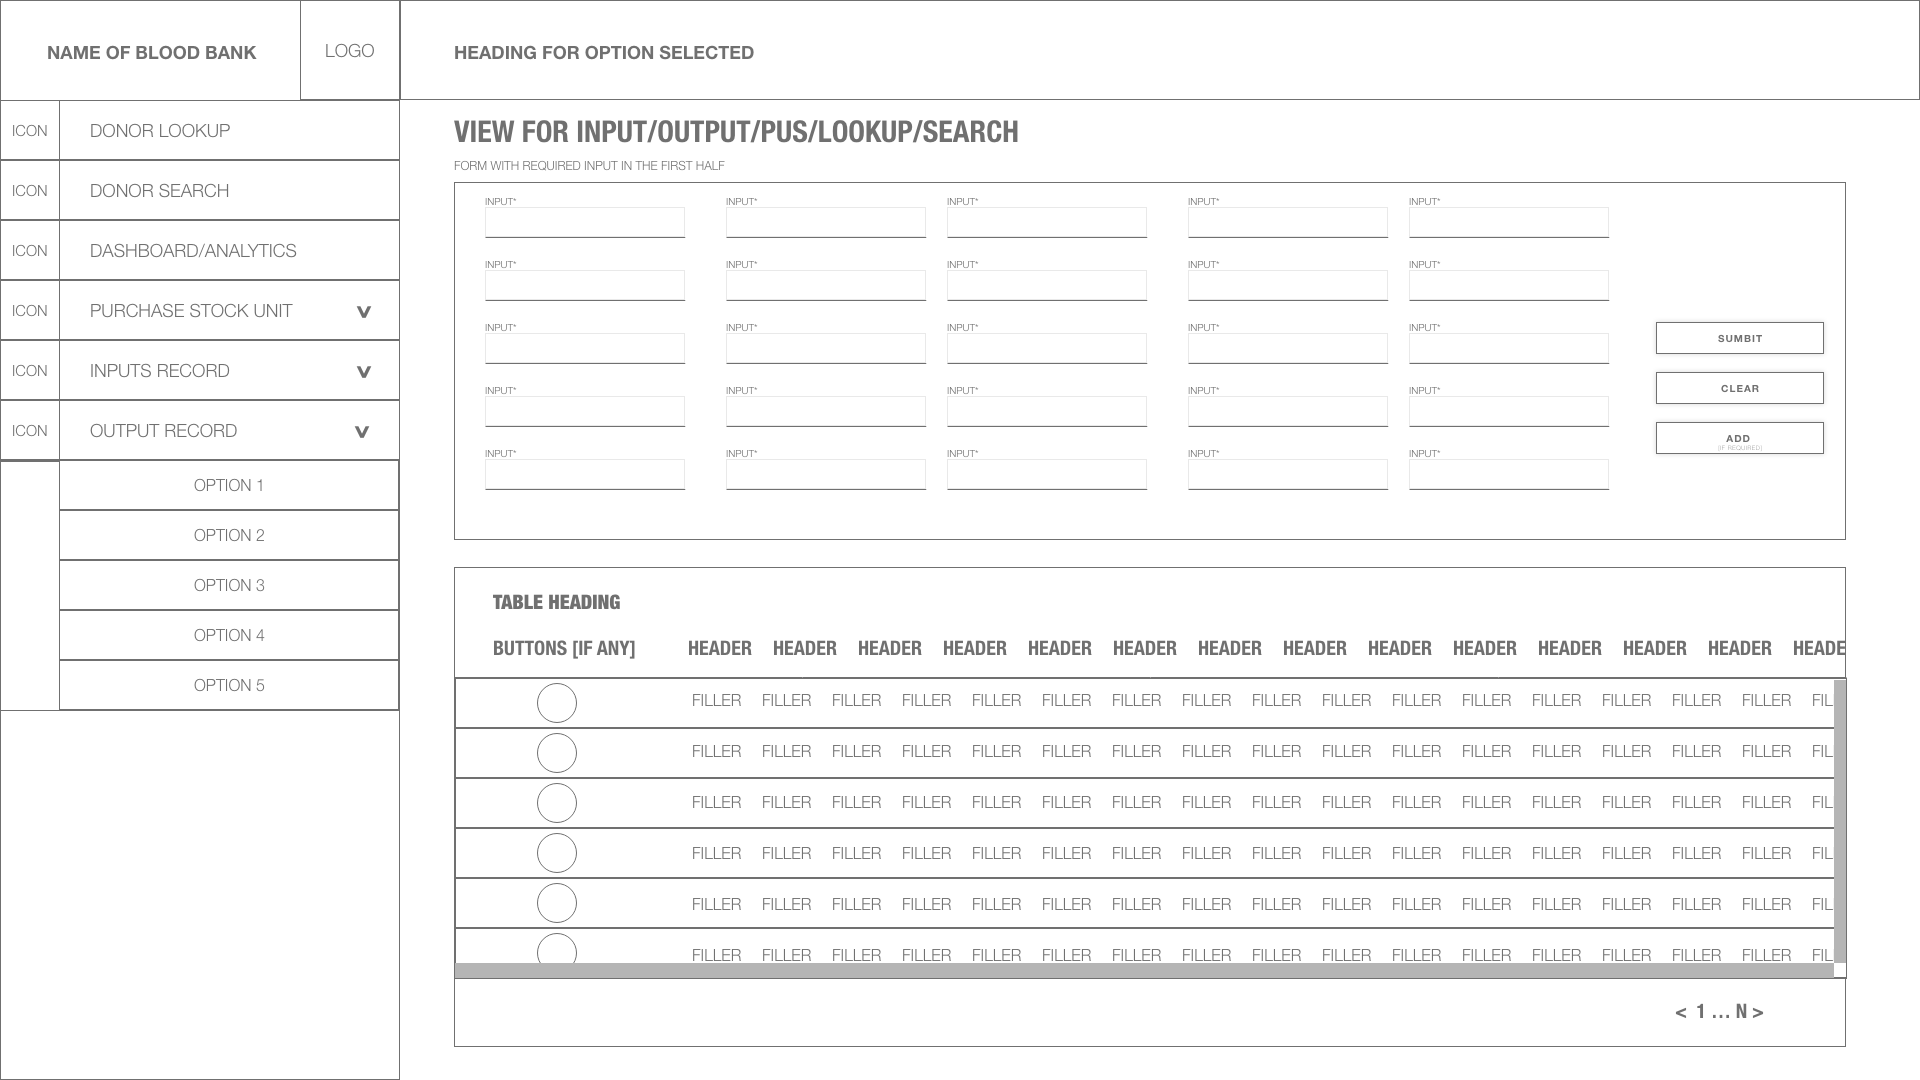
\includegraphics[scale=0.2]{wireframe1.png}
	\caption{Wireframe 1}
\end{figure}
The first wireframe shows the view for the various modules including Input, Output, \ac{PUS}, Lookup and Search. The approach was simple with drop-down lists and a table showing all the results. A sidebar for navigating throughout the application.\par
\begin{figure}[h!]
	\centering
	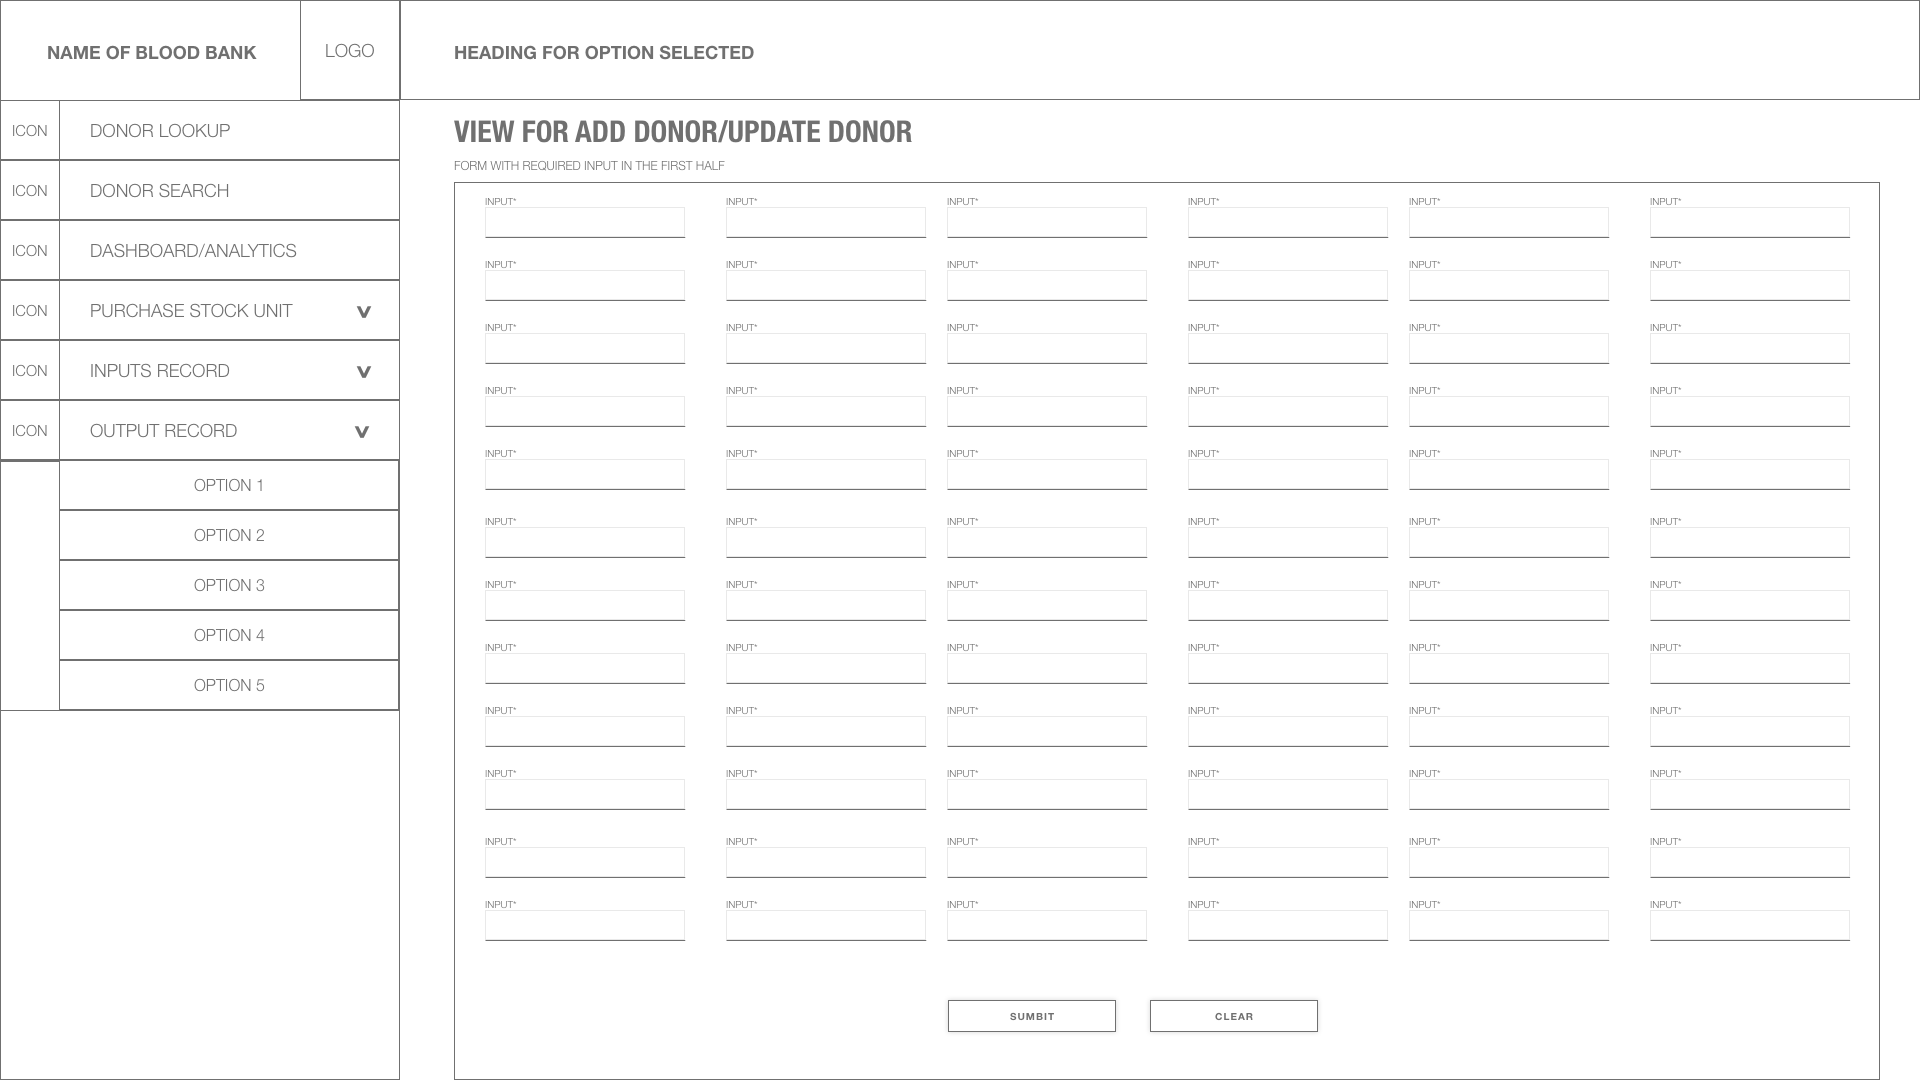
\includegraphics[scale=0.2]{wireframe2.png}
	\caption{Wireframe 2}
\end{figure}
The second wireframe shows the add/update donor form, with various fields to be provided to complete the record or update the donor details.\par
\begin{figure}[h!]
	\centering
	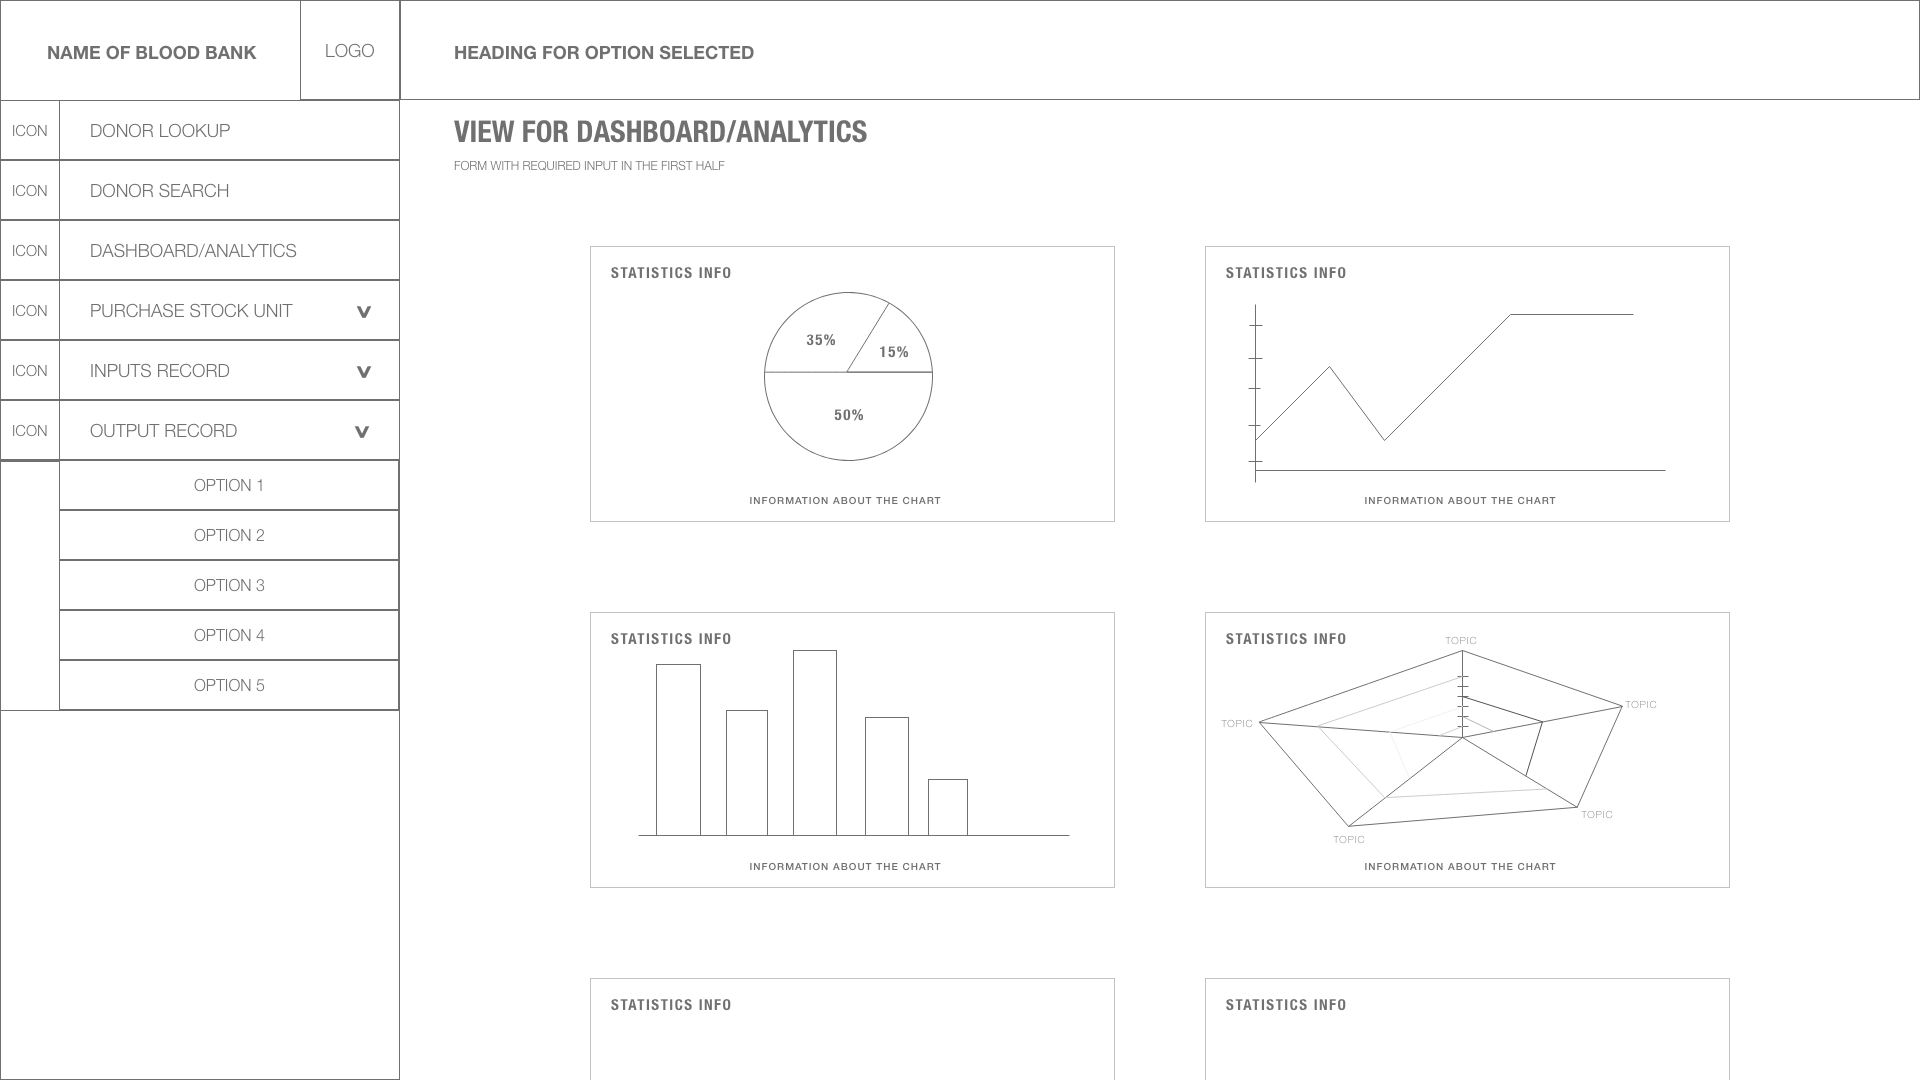
\includegraphics[scale=0.2]{wireframe3.png}
	\caption{Wireframe 3}
\end{figure}
The third wireframe showcases the dashboard/analytics page of the Blood Bank which will be used to view various \ac{KPI}(s) of the Blood Bank. This module incorporates various charts and graphs and the objective was to provide a user interface in which an individual could take a glance of the whole system with just a click of the button.
\subsection{Database Design}
We were given real register record pages courtesy of Rotary Blood Bank. Using these records, identification of database tables and their fields was done. The objective was to reduce redundancy and remove any fields which can be automatically filled such as calculation of age from the \ac{DOB} of the donor.\par
Looking at the table and their fields, they have a tendency to change over time with newer fields as per the needs of a Blood Bank. Using a SQL database could have been a very tedious and time taking work, also resolving issues would be very difficult in such a complex system.\par
\subsubsection{NoSQL Database}
NoSQL which stands for "Not only SQL" is a non-relational database that allows for storage and retrieval of data. NoSQL database includes simplicity of style, less complicated horizontal scaling to clusters of machines and finer management over handiness. the information structures utilized by NoSQL databases are totally different from those utilized by default in relative databases that makes some operations quicker in NoSQL. The quality of a given NoSQL information depends on the matter it ought to solve. Knowledge structures utilized by NoSQL databases are typically conjointly viewed as additional versatile than on-line database tables. The choice of NoSQL database was MongoDB because of it's versatile nature and better community. \cite{gfg_nosql} \newline
	
\begin{table}[H]
	\begin{center}
		\label{tab:table1}
		\begin{tabular}{l|c|c}
			\textbf{S.No.} & \textbf{NoSQL} & \textbf{SQL} \\
			\hline
			1. & Non relational database. & Relational database. \\
			2. & Document based. & Table based. \\
			3. & Dynamic schema for unstructured data. & Predefined schema for structured data. \\
			4. & Horizontally scalable. & Vertically scalable. \\
		\end{tabular}
	\end{center}
\caption{NoSQL vs SQL}
\end{table}
	
\subsubsection{Creation of collections}
In MongoDB a table is called a collection. Using the given record we identified each column for the database and created an excel sheet out of it. These excel sheets were then validated by the personnel at the Blood Bank, upon their validation, we proceeded with the creation of the actual collection for the database.\par
\begin{figure}[H]
	\centering
	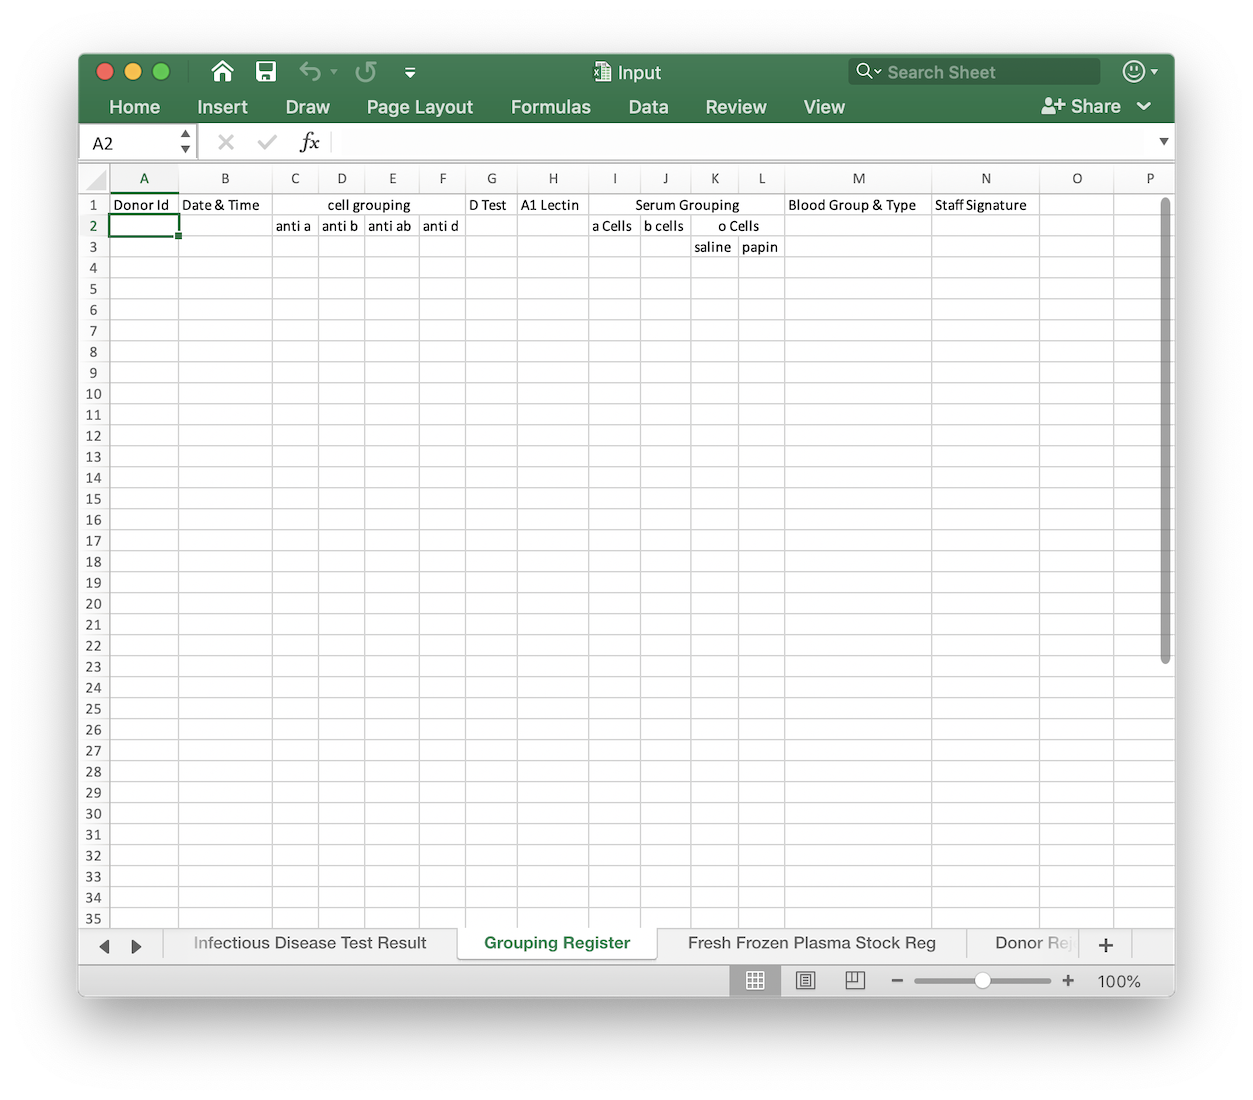
\includegraphics[scale=0.65]{excel.png}
	\caption{Input Excel Sheet}
\end{figure}
\begin{figure}[H] 
	\centering
	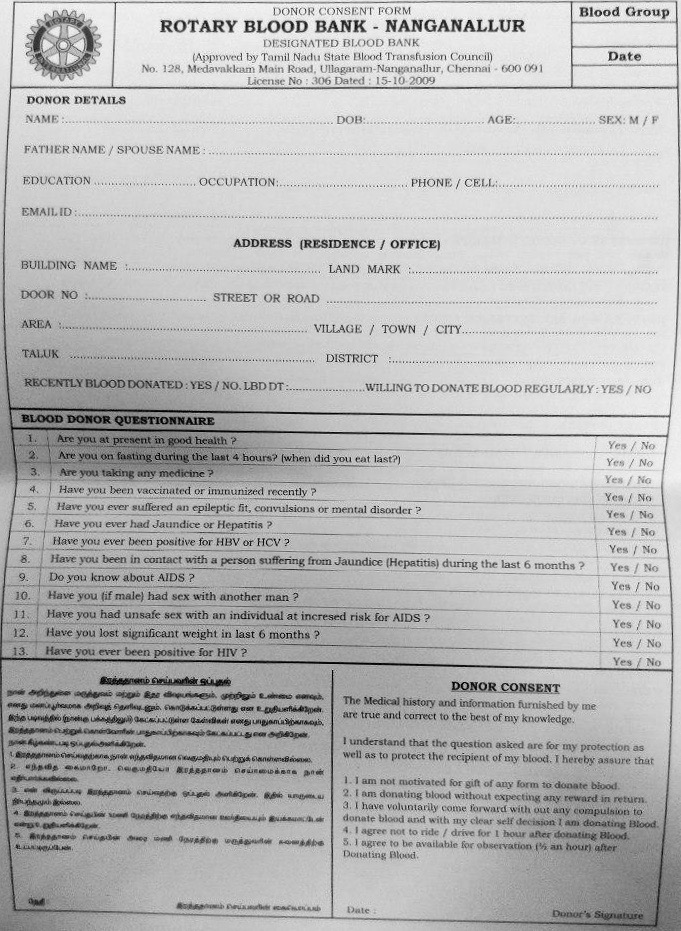
\includegraphics[scale=0.63]{register_page.jpeg}
	\caption{Donor Consent Form}
\end{figure}
\begin{figure}[H]
	\centering
	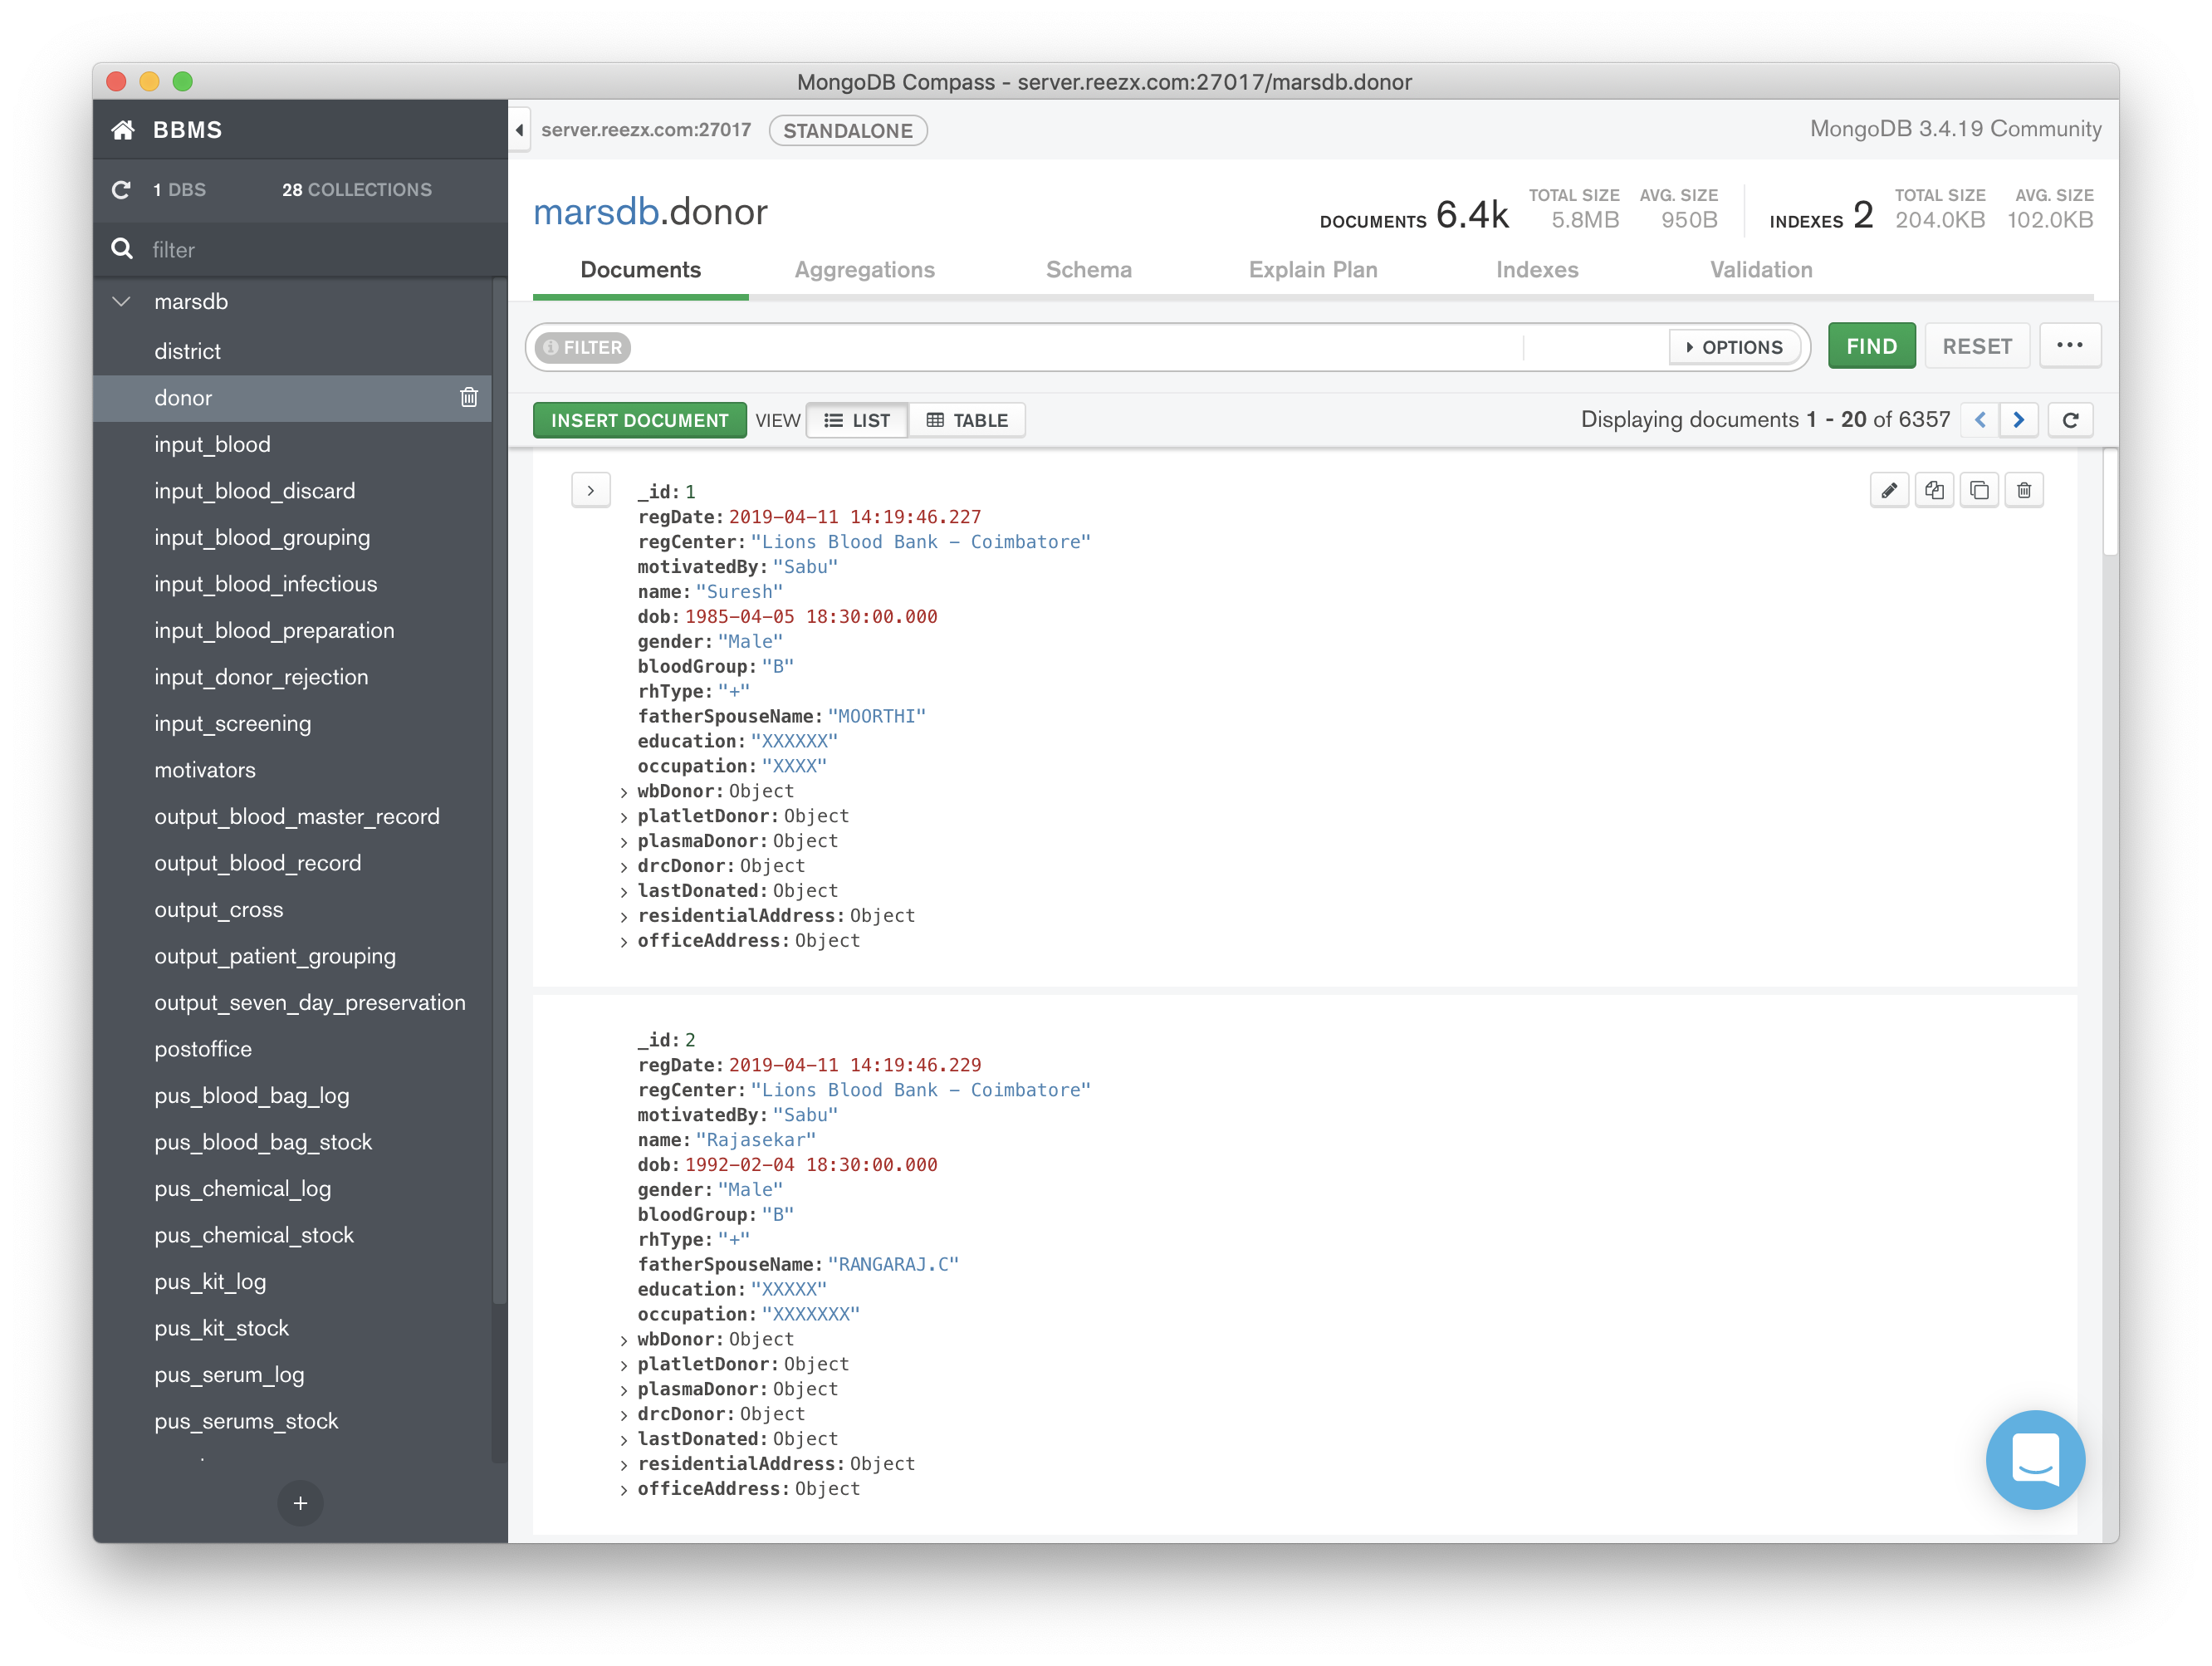
\includegraphics[scale=0.32]{mongo_compass.png}
	\caption{MongoDB Compass showing various collections and documents}
\end{figure}
The data is stored in the form of \ac{JSON}, in MongoDB. All the data in collections is known as documents and unlike SQL we can have independent fields.

\subsection{Modules}
\subsubsection{a. Search}
The donor's info is stored in registers and looking for donors when needed is very time taking. By storing the donor's info and details into a centralized database we can easily search using donor id or donor details. If upon search a donor is not found we can add the donor using the same details as well, which is very convenient and fast for the blood bank. Figure 4.7, 4.8 represents the data models for the user's address and blood bank document stored in the database.
\begin{figure}[H]
	\centering
	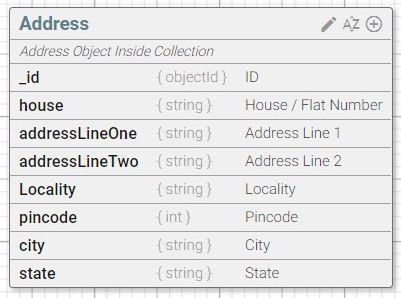
\includegraphics[scale=0.6]{search_address.jpeg}
	\caption{Address Data Model}
\end{figure}
\begin{figure}[H]
	\centering
	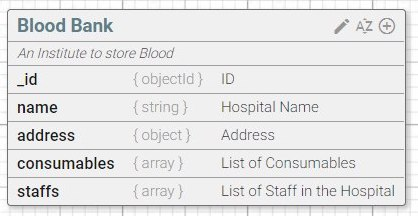
\includegraphics[scale=0.6]{search_blood_bank.jpeg}
	\caption{Blood Bank Data Model}
\end{figure}

\subsubsection{b. Lookup}
The donor's info is stored in registers and looking for donors when needed is very time taking. By storing the donor's info and details into a centralized database we can easily search using advanced query. In this module, the implementation to print the data of the query result is also a very convenient way to present the lists of donors. The advanced query include - 'Blood group, Rh factor, Gender, Donor type,  Area, etc'. Figure 4.9 represents the data model for the user document stored in the database.
\begin{figure}[H]
	\centering
	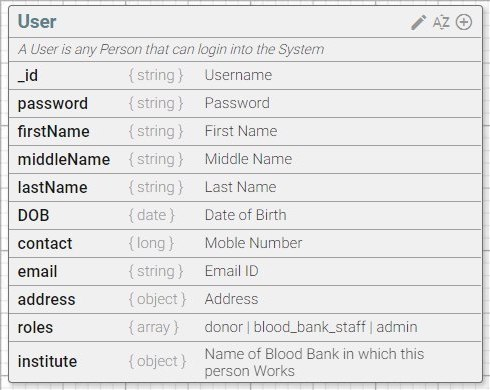
\includegraphics[scale=0.6]{lookup_user.jpeg}
	\caption{User Data Model}
\end{figure}

\subsubsection{c. Input}
This module is to maintain details of blood donated to the blood bank by donors and the various tests that are carried out after a donation, prior to storing the blood. A lot of registers and logs are to be maintained for the same which is a very tiring and tedious work to do and auditing for the same is also not possible. Through our system and database, everything can be simplified and easy to manage and view everything. The goal here is to reduce all the manual entry and simplify the process of data entry and retrieval. Figure 4.10 - 4.13 represents various data models used for this module's document storage in the database.
\begin{figure}[H]
	\centering
	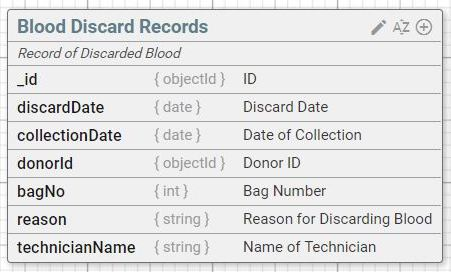
\includegraphics[scale=0.6]{input_blood_discard_rec.jpeg}
	\caption{Blood Discard Data Model}
\end{figure}
\begin{figure}[H]
	\centering
	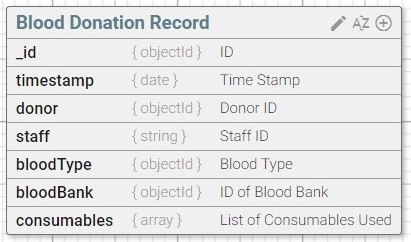
\includegraphics[scale=0.6]{input_blood_donation.jpeg}
	\caption{Blood Donation Data Model}
\end{figure}
\begin{figure}[H]
	\centering
	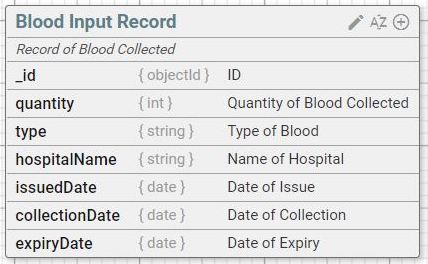
\includegraphics[scale=0.6]{input_blood_input_record.jpeg}
	\caption{Blood Input Record Data Model}
\end{figure}
\begin{figure}[H]
	\centering
	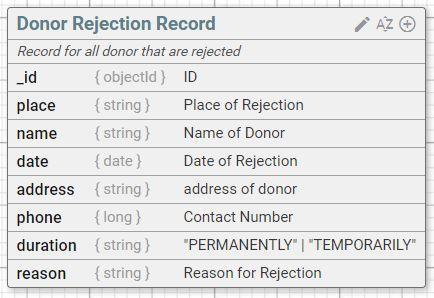
\includegraphics[scale=0.6]{input_donor_rejection.jpeg}
	\caption{Donor Rejection Data Model}
\end{figure}

\subsubsection{d. Output}
This module is to maintain details of blood issued by the blood bank to patients and the various tests that are carried out on the stored the blood, prior to an issue. A lot of registers and logs are to be maintained for the same which is a very tiring and tedious work to do and auditing for the same is also not possible. Through our system and database, everything can be simplified and easy to manage and view everything. The goal here is to reduce all the manual entry and simplify the process of data entry and retrieval. Figure 4.14 represents the stock register data models used for the document storage in the database.
\begin{figure}[H]
	\centering
	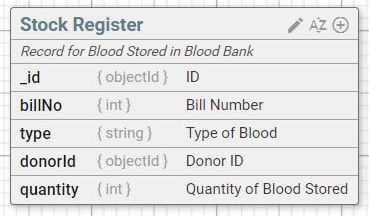
\includegraphics[scale=0.6]{output_stock_reg.jpeg}
	\caption{Stock Register Data Model}
\end{figure}

\subsubsection{e. \ac{PUS}}
This module is to maintain the stock status of various consumables used in a blood bank like a blood bag, needles, syringes, cotton, chemicals etc. There is no digital way of getting to know the exact quantity of all the items. Our system offers a method of inventory management in which we provide digitally all the present items available and offer interactive screens in which we can add/remove new items. Auto logging of all the transactions of adding and removal of items is done in the backend. Saving time and reducing overhead work. Figure 4.15 - 4.19 represents various data models used for this module's document storage in the database.
\begin{figure}[H]
	\centering
	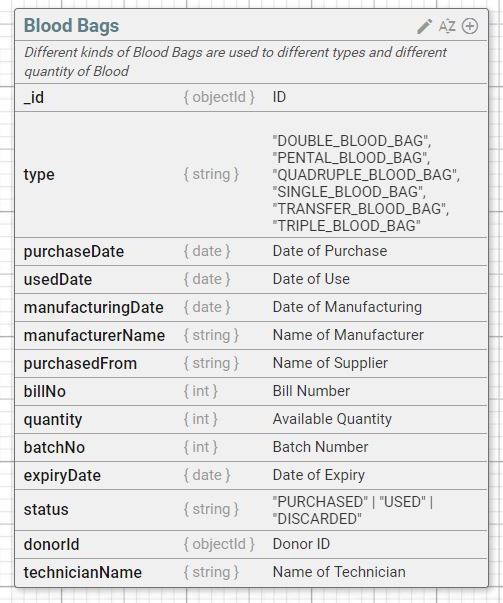
\includegraphics[scale=0.6]{pus_blood_bags.jpeg}
	\caption{Blood Bags Data Model}
\end{figure}
\begin{figure}[H]
	\centering
	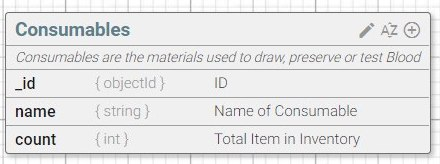
\includegraphics[scale=0.6]{pus_consumables.jpeg}
	\caption{Consumables Data Model}
\end{figure}
\begin{figure}[H]
	\centering
	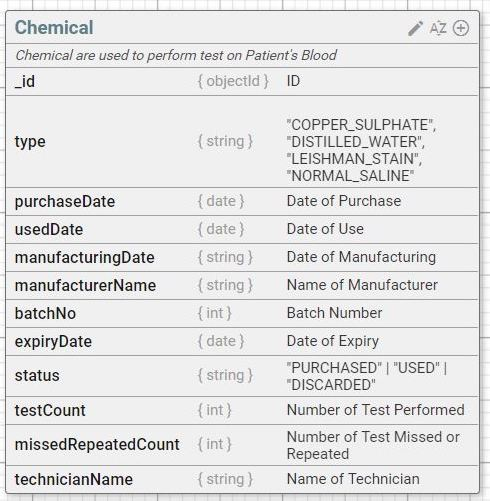
\includegraphics[scale=0.55]{pus_chemical.jpeg}
	\caption{Chemicals Data Model}
\end{figure}
\begin{figure}[H]
	\centering
	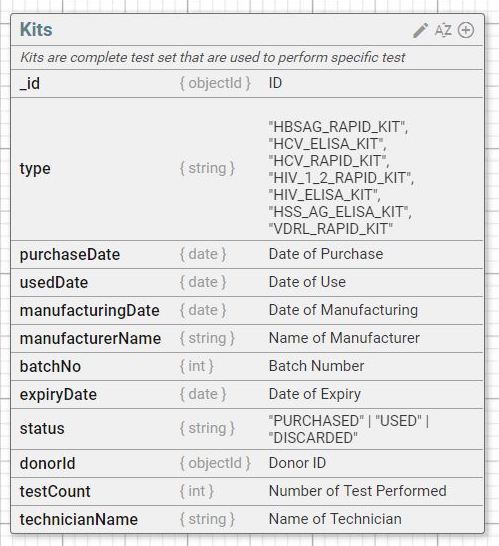
\includegraphics[scale=0.55]{pus_kits.jpeg}
	\caption{Kits Data Model}
\end{figure}
\begin{figure}[H]
	\centering
	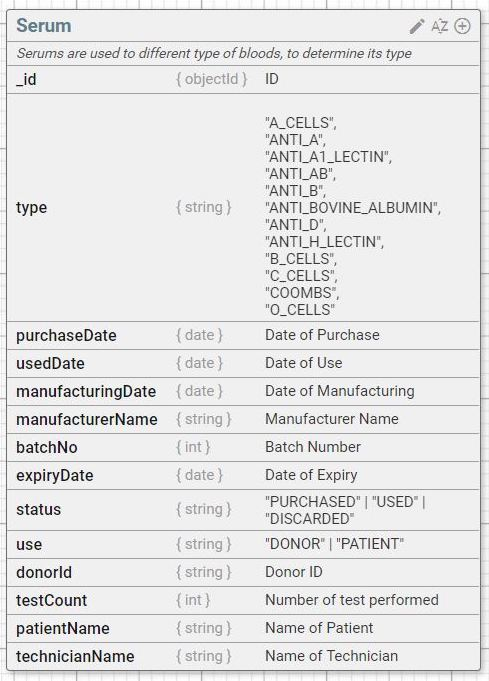
\includegraphics[scale=0.6]{pus_serum.jpeg}
	\caption{Serums Data Model}
\end{figure}

\section{Logical Design}
\section{RESTful API}
RESTful API is a piece of program which is an \ac{API} which uses \ac{HTTP} to GET, PUT, DELETE and POST data. They are usually know as RESTful web service which is based on \ac{REST} technology, which is an approach of architectural style for communication often used in web development.

\subsection{UML Diagrams}
\cite{uml_ref}
\subsubsection{a. Use Case Diagram}
\begin{figure}[H]
	\centering
	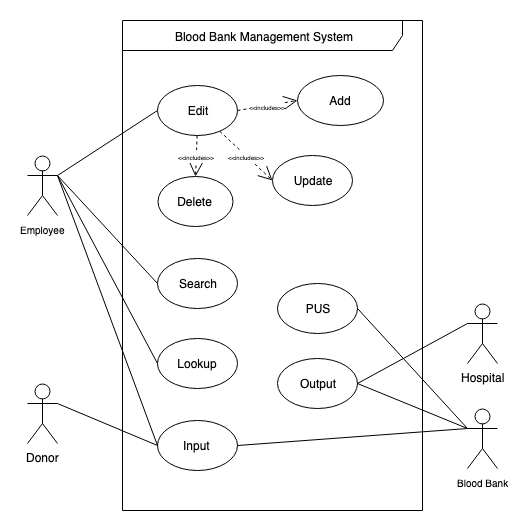
\includegraphics[scale=0.7]{usecase.png}
	\caption{Use Case Diagram}
\end{figure}

\subsubsection{b. Sequence Diagram}
\begin{figure}[H]
	\centering
	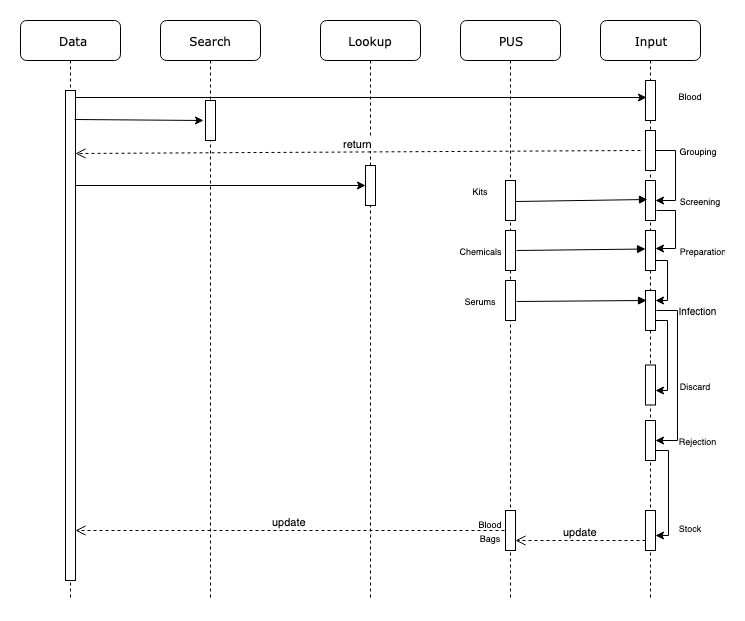
\includegraphics[scale=0.6]{sequence.png}
	\caption{Sequence Diagram}
\end{figure}

\subsubsection{c. Flow Diagram}
\begin{figure}[H]
	\centering
	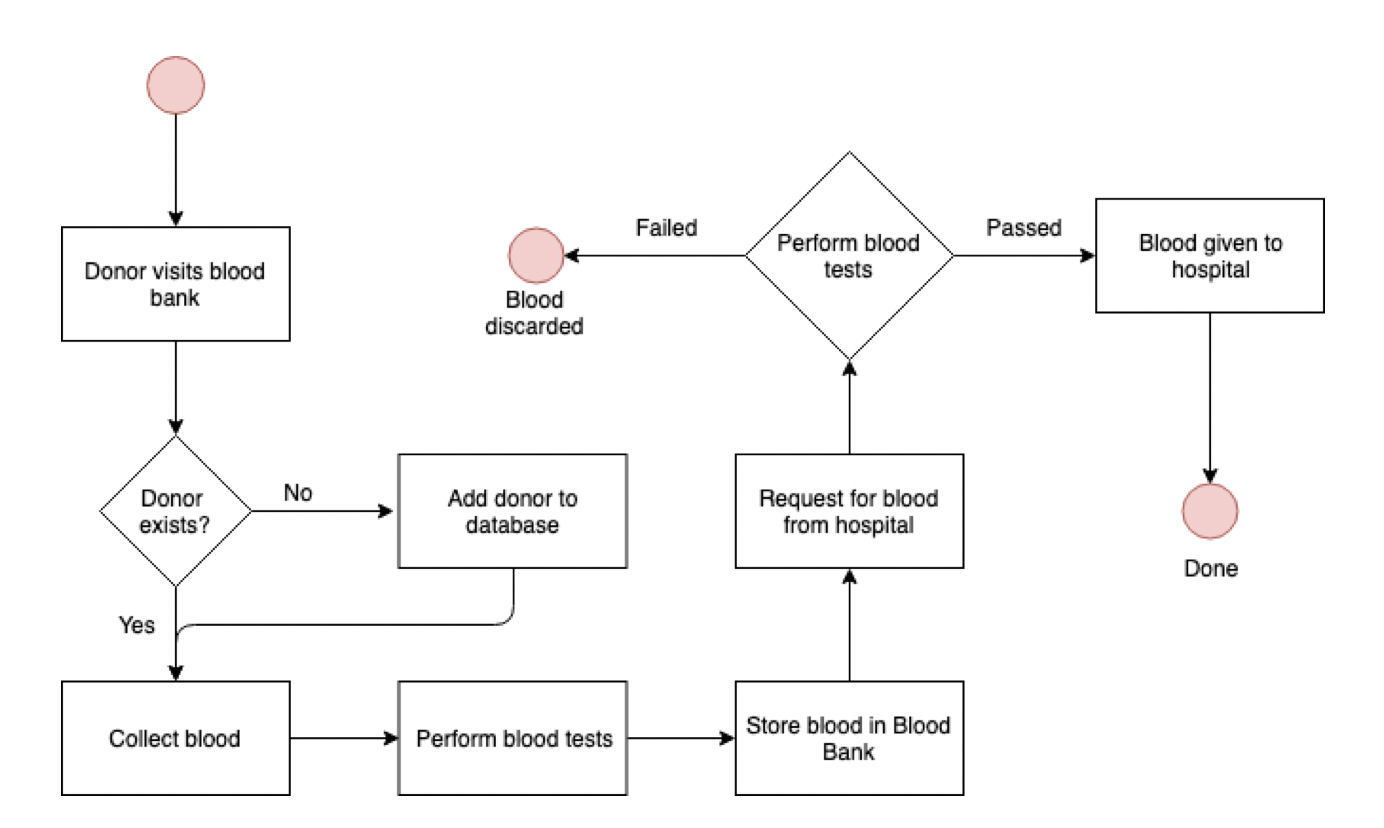
\includegraphics[scale=0.6]{flow_diag.png}
	\caption{Flow Diagram}
\end{figure}

\chapter{Testing}
\section{Testing Objectives}
The purpose of testing is to discover errors. Testing is the process of trying to discover every conceivable fault or weakness in a product. It provides a way to check the functionality of components, sub-assemblies, assemblies and/or a finished product. It is the process of exercising software with the intent of ensuring that the software system meets its requirements and user expectations and does not fail in an unacceptable manner. There are various types of test. Each test type addresses a specific testing requirement. \cite{testing_book}
\section{Types of tests}
\subsection{Unit Testing}
Unit testing involves the design of test cases that validate that the internal program logic is functioning properly and that program inputs produce valid outputs. All decision branches and internal code flow should be validated. It is the testing of individual software units of the application. It is done after the completion of an individual unit before integration. This is structural testing, that relies on knowledge of its construction and is invasive. Unit tests perform basic tests at the component level and test a specific business process, application, and/or system configuration. Unit tests ensure that each unique path of a business process performs accurately to the documented specifications and contains clearly defined inputs and expected results.
\subsection{Integration Testing}
Integration tests are designed to test integrated software components to determine if they actually run as one program. Testing is event-driven and is more concerned with the basic outcome of screens or fields. Integration tests demonstrate that although the components were individually satisfaction, as shown by successfully unit testing, the combination of components is correct and consistent. Integration testing is specifically aimed at exposing the problems that arise from the combination of components.
\subsection{Functional Testing}
Functional tests provide systematic demonstrations that functions tested are available as specified by the business and technical requirements, system documentation, and user manuals.
Functional testing is centered on the following items:
\newline
\textbf{Valid Input:} Identified classes of valid input must be accepted.
\newline
\textbf{Invalid Input:} Identified classes of invalid input must be rejected.
\newline
\textbf{Functions:} Identified functions must be exercised.
\newline
\textbf{Output:} Identified classes of application outputs must be exercised.
\newline 
\textbf{Procedures:} Interfacing systems or procedures must be invoked
\par
Organization and preparation of functional tests are focused on requirements, key functions, or special test cases. In addition, systematic coverage pertaining to identify business process flows, data fields, predefined processes, and successive processes must be considered for testing. Before functional testing is complete, additional tests are identified and the effective value of current tests is determined.
\subsection{Acceptance Testing}
User Acceptance Testing is a critical phase of any software and it requires significant participation by the end user. It also ensures that the system meets all the functional requirements.
\subsection{System Testing}
System testing ensures that the entire integrated software system meets requirements. It tests a configuration to ensure known and predictable results. An example of system testing is the configuration oriented system integration test. System testing is based on process descriptions and flows, emphasizing pre-driven process links and integration points.
\subsection{White Box Testing}
White Box Testing is a testing in which the software tester has knowledge of the inner workings, structure and language of the software, or at least its purpose. It is a purpose. It is used to test areas that cannot be reached from a black box level.
\subsection{Black Box Testing}
Black Box Testing is testing the software without any knowledge of the inner workings, structure or language of the module being tested. Black box tests, like most other kinds of tests, must be written from a definitive source document, such as specification or requirements document, such as specification or requirements document. It is a testing in which the software under test is treated, as a black box you cannot “see” into it. The test provides inputs and responds to outputs without considering how the software works.
\subsection{Alpha Testing}
In software development, the alpha test will be a test among the teams to confirm that your product works. Originally, the term alpha test meant the first phase of testing in a software development process. The first phase includes unit testing, component testing, and system testing. It also enables us to test the product on the lowest common denominator machines to make sure download times are acceptable and preloads work.
\subsection{Beta Testing}
In software development, a beta test is the second phase of software testing in which a sampling of the intended audience tries the product out.
\section{Tests Strategy and Approach}
As we can see the importance of testing in an application. The following test cases were kept in mind keeping the user at the center.
\subsection{Test Objective}
1. Maintain the application's integrity and robustness.
\newline
2. Database transactions are complete and there is no data loss or redundancy.
\newline
3. Proper prompt and error messages are displayed.
\newline
4. The data from the forms are validated properly before storing in the database.
\subsection{Features to be tested}
1. All the modules serve their purpose as intended.
\newline
2. All the forms have all the specified fields required for data collection.
\newline
3. Verify the entries are in correct format and there are no duplicate entries.
\newline
4. Navigation across the application is meaningful and states are properly maintained.

\chapter{Conclusion}
This project is made with a sense of doing better towards the problems that are faced by the blood bank management inventories and helping society. A web application is made to ensure that this system is malleable and thus can sustain for a long time. The \ac{MERN} technology stack is used to achieve these goals. To achieve the goals we have been working for the rotary blood bank and getting their feedback to improve our system the end users. Apart from the basic features of a database i.e Add, Search, Update, and Delete, we are providing the offline mode and analytics. The extensive amount of data that is handled, this gives precise analytics. We have made the process of auditing less cumbersome and reduced data redundancy.\par
The analytics are made through several key index points that are available some of them are the total donor count, classification on the basis of blood count, classification on the basis of the region where the blood was donated, the ratio of male to the female population, and motivation.\par
A standardized time-efficient and sustainable inventory management system has been provided to the Rotary Blood Bank.


\chapter{Future Enhancement}
The current project can be enhanced for future use cases with the following pointers that are available.
\section{Exception rate}
The future analysis can include the error count of the people and their causes of death. An example would be to check if there was a delay in searching or delivery of the blood or whether the blood was not available. This analysis will help the system evaluate its most prominent flaws and tackle them.
\section{Donor location}
The application can be extended to the donors and if the need for blood arises users in the vicinity must be informed and allowed to donate blood. The users must be filtered on the basis of requirements and only a select number of candidates must get the message. This can also have logistics of whether the blood reached to patient or not. This will help the system to complete the cycle of blood donation.
\section{Banks closet}
The system can expand to accommodate the hospital and allow them to look upon the blood bank near them and request blood at all times. This can include the ambulances to help track the nearest blood bank and request for blood in case of vital accidents and emergency situations.
\section{Notifications}
The hospital if included must have a facility to notify the donors and the blood bank about its requirements and the priority level of the blood that is to be used. The blood banks must also know all the hospitals that are near to their hospital.
\section{Register to digital}
An obvious part is to make the input easier to shift from the registers to the digital format. This can be achieved using Machine Learning and Image Processing. We can use the Otsu Binarization Technique along with a NN to recognize handwriting.


%%%%%%%%%%%%%%%%%%%%%%%%%%%%%%%%%%%%%%%%%%%%%%%%%%%%%%%%%%%%
% Appendices.

\appendix
\chapter{Otsu Binarization Thresholding}
Otsu Binarization is a technique that is accustomed used to convert grayscale images to monochrome is one of the many binarization methods.
This technique aims to find the threshold value where the sum of spread is minimum. It minimizes the grey levels of an image. Otsu’s thresholding technique involves iterating all possible values of threshold and calculating the measure of the spread for pixel level that falls in foreground and background.

This method requires the exhaustive scratch of values that maximize the interclass variance, that is the weighted sum of variances between two classes. The objective is to minimize the interclass variance.

The algorithm assumes that the image contains two classes of pixels following bi-modal histogram, it then calculates the optimum threshold separating the two classes so that their combined spread is minimal.

\section{The Mathematics}
We exhaustively search for the threshold, defined as a weighted sum of variances of the two classes:
\begin{equation}
\sigma^{2}_{\omega}(t) = \omega_{0}(t) \sigma^{2}_{0}(t) + \omega_{1}(t) \sigma^{2}_{1}(t) 
\end{equation}
Weights $\omega_{0}$   and  $\omega_{1}$ are the probabilities of the two classes separated by a threshold t, and  $\sigma^{2}_{0}$ and $\sigma^{2}_{1}$ are variances of two classes The class probability $\omega_{0,1}(t) $ is computed from the L bins of the histogram:
\begin{equation}
\omega_{0}(t) = \sum_{i=1}^{t-1} p(i)
\end{equation}
\begin{equation}
\omega_{1}(t) = \sum_{i=t}^{L-1} p(i)
\end{equation}
Otsu demonstrates that minimizing the intra-class variance is the same as maximizing inter-class variance as shown by the equation :
\begin{equation}
\sigma^{2}_{b}(t) = \omega_{0}(t) \omega_{1}(t) [\mu_{0}(t)-\mu_{1}(t)]^{2}
\end{equation}
That is expressed in terms of probabilities $\omega$ and means $\mu $ . Keeping the class mean as  $\mu_{0,1,T}(t)$ is:
\begin{equation}
\mu_{0}(t) = \frac  {\substack{\sum_{i=0}^{t-1} ip(i)}}
{\substack{\omega_{0}(t)}  }
\end{equation}
\begin{equation}
\mu_{1}(t) = \frac  {\substack{\sum_{i=t}^{L-1} ip(i)}}
{\substack{\omega_{1}(t)}  }
\end{equation}
\begin{equation}
\mu_{T} = \sum_{i=0}^{L-1} ip(i)
\end{equation}
These can be verified:
\begin{equation}
	\omega_{0} + \omega_{1} = 1
\end{equation}
The class probabilities and class 
means should be computed at all turns.

\section{The algorithm that can be implemented}
There is a four-step algorithm.
\newline
\textbf{Step 1:} Make a histogram and probabilities for each intensity
\newline
\textbf{Step 2:} Set up the initial $\omega_{i}(0)$ and $\mu_{i}(0)$.
\newline
\textbf{Step 3:} Step through all possible thresholds from t=1…..maximum intensity.
\newline
\textbf{Step 3.1:} Update $\omega_{i}$ and $\mu_{i}$.
\newline
\textbf{Step 3.2:} Compute $\sigma^{2}_{b}(t)$.
\newline
\textbf{Step 4:} The desired threshold corresponds to the maximum of $\sigma^{2}_{b}(t)$.

\section{Availability}
The implementation can be done in any language which facilitates mathematics. It is advised to use Matlab, Octave or Python for implementation. The OpenCV library has an inbuilt implementation of Otsu Binarization technique.

%%%%%%%%%%%%%%%%%%%%%%%%%%%%%%%%%%%%%%%%%%%%%%%%%%%%%%%%%%%%
% Bibliography.
\bibliography{references}
%%%%%%%%%%%%%%%%%%%%%%%%%%%%%%%%%%%%%%%%%%%%%%%%%%%%%%%%%%%%
\end{document}
